\section{Introduction}

Depuis que la naissance de l'informatique, l'humain a toujours convoité l'idée de pouvoir intéragir verbalement avec un ordinateur, et ce, de manière transparente comme s'il s'agissait d'un autre humain apte à capter la majorité des nuances du discours entretenu. Bien que ce sujet aura fait couler beaucoup d'encre et fait tourner les têtes, il n'existe toujours pas à ce jour une formule secrète parfaite pour parvenir à sa réalisation. Au cours des années, différentes démarches ont été proposées. Traditionnellement, des approches algorithmiques étaient favorisées et certains projets se fondent encore sur ces dernières, tel que \textbf{Watson} de \textbf{IBM}, créé en 2011 \cite{ibmWatson}. Ces approches ont toutefois le défaut d'être longues et ardues à développer. De plus, la réutilisation des travaux sous-jacents est plus complexe en raison du caractère sur mesure et classique du problème, en lien avec le champ d'application spécifique auquel il s'applique, tel que de jouer à Jeopardy. Ce type d'approche classique est en processus d'être changé par des approches fonctionnant par réseaux de neurones profonds déjà depuis 2014, le point marquand de ce virage étant la découverte des mécanismes d'attention dans les réseaux de neurones profonds par Bahdanau et al. en 2014 \cite{attentionMechanism}.  \\
%EDIT: je parlerais d’IBM Watson, mais c’est une approche classique et c’est pas neuronal. C’est du 2014-2015, thought, donc ça se placerait bien dans l’intro. Faudrait trouver un de leurs papers ici, mais ça paraît que toute leur shit c’est des algos classiques, c’est décevant de leur part: http://researcher.watson.ibm.com/researcher/view_group_pubs.php?grp=2099

Ainsi, récemment, des approches mettant en jeu des réseaux de neurones artificiels ont leur apparition et ont immédiatement connus beaucoup de succès. Le grand pas réalisé en 2014 fait en sorte que les techniques par réseaux de neurones profonds viennent à dépasser les performances des techniques classiques pour la tâche de faire de la traduction automatique \cite{attentionMechanism}, tels qu'illustrés dans la  \autoref{fig:attn}. C’est de tels systèmes qui sont désormais utilisés chez \textbf{Google} pour la mise en production du fameux \textbf{Google Translate} \cite{googleTranslate}, avec leur publication officielle d'une amélioration de cette architecture neurale plus tard en octobre 2016. Cette même compagnie utilise aussi des algorithmes de \textit{Speech-to-Text} tels que tels que celui de William Chan et Ian Lane \cite{acousticModeling} afin de pouvoir générer des sous-titres automatiquement pour de l'audio ou des vidéos (tels que \textbf{YouTube} le fait avec des recherches similaires) et afin de pouvoir analyser les vidéos et les lier entre elles avec une approche sémantique. \\

\begin{figure*}
  \centering
  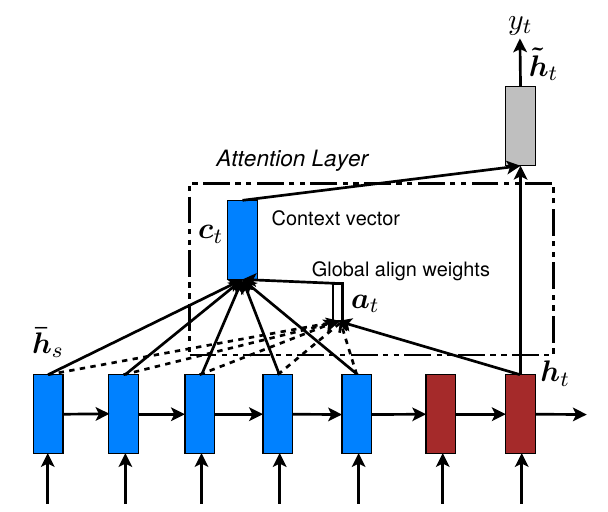
\includegraphics[width=\textwidth, height=0.4\textheight, keepaspectratio]{bahdanauAttentionMechanism2014}
  \caption{Mécanisme d'attention sous sa forme générale, tel qu'introduit par Bahdanau et al. en 2014 \cite{attentionMechanism}. En premier lieu, le texte est lu séquentiellement en entrée (en bas à gauche). Ensuite, une requête est faite pour filtrer ce qui est lu et faire l'alignement d'attention (en bas à droite). Cette requête est comparée à toute l'information à filtrer par le mécanisme d'attention (au centre). Ensuite, un résultat est formulé par un calcul neuronal sur le mécanisme d'attention et en fonction de la requête demandée (en haut).}
  \label{fig:attn}
\end{figure*}

Il ne s'agit ici que de différents morceau de puzzle qui peuvent mener à la création d'un agent conversationnel complètement basé sur ces meilleurs systèmes par réseaux de neurones. La création d'un tel agent est une tâche compliquée dû au fait qu'il faut assembler les découvertes des différentes parties, l'une des raisons pourquoi le mouvement open-source est si proéminent, menant vers une convergence. Dans le cadre d'un échange verbal entre deux êtres, une multitude de tâches sont accomplies sans même que nous ne soyons conscient. Le tout débute lors d'un contact initial le plus souvent dans une forme auditive vers un destinataire. En partant de ce point, à titre de destinataire, il faut premièrement capter le message et l'interpréter en mots. Malgré des obstacles environnants et culturels variés réduisant la qualité de cette réception, filtrer ce qui est réellement important dans le signal et le décoder selon un dialecte particulier est la première étape, ici s'insère les architectures de \textit{Speech-to-Text}. Une fois en possession de ce message, il faut établir des liens entre l'énoncé qui a été donné et un registre de connaissances (tel que Wikipédia par exemple), ainsi que les liens avec les discussions passées avec le même interlocuteur. C'est alors qu'il est possible d'établir la réponse la plus appropriée compte tenu d'une panoplie de facteurs comme l'identité de notre interlocuteur, son domaine de travail et son niveau d'éducation, des valeurs d'intérêt global et nos connaissances, et ainsi de suite. Cette phase implique des réseaux de neurones capables d'analyser du texte à partir d'une requête, tels que les systèmes basés sur des améliorations et une exploration des mécanismes d'attention \cite{attentionBasedApproaches} ensuite appliquées à cette nouvelle tâche, introduits dans les travaux de Karl Moritz Hermann et al. chez Google, ainsi en 2015 \cite{readNcomprehend}. L'attention étant bien portée dans le texte, il est ensuite possible de générer une réponse, tel qu'avec les recherches récentes de Iulian Serban et al. déjà en 2016 \cite{chatbot\string:HRED} et maintenant en 2017 \cite{chatbot\string:LVHRED}.\\

Une fois cette réponse textuelle en main, il ne reste qu'à la traduire en audio, ce qui est dorénavant possible de générer en temps réel avec une approche par réseaux de neurones convolutionnels tels que Wavenet \cite{wavenet}, ici encore développé chez Google pour faire du \textit{Text-to-Speech}, l'inverse du \textit{Speech-to-Text}. L'un des obstacles à cela est lorsque les utilisateurs possèdent un accent fortement prononcé et qui est unique, et la différences dans les langues. Du moins, ce genre de systèmes est adaptable à plusieurs langues, et au moment où du texte est en possesion, il est possible de le traduire automatiquement. Au final, cela demande beaucoup de données d'apprentissage. Pour rajouter encore plus de difficulté, ces étapes sont à faire dans un interval de temps très rapide pour éviter les longs délais. Heureusement, l'étape la plus longue est de faire apprendre aux réseaux de neurones ce qu'ils ont à apprendre. Ils sont ensuite très performants lors de l'étape d'inférence, où ils analyse et génèrent réellement de l'information en production. \\
